\documentclass[11pt]{article}
\usepackage{amsmath}
\usepackage{physics}
\usepackage{amssymb}
\usepackage{graphicx}
\usepackage{hyperref}
\usepackage{amsfonts}
\usepackage{cancel}
\usepackage{xcolor}
\hypersetup{
	colorlinks,
	linkcolor={black!50!black},
	citecolor={blue!50!black},
	urlcolor={blue!80!black}
}
\usepackage{newpxtext,newpxmath}
\usepackage[left=1.25in,right=1.25in,top=0.9in,bottom=0.9in]{geometry}
\usepackage{framed}
\usepackage{caption}
\usepackage{subcaption}

%\newcommand{\fig}[1]{figure #1}
%\newcommand{\explain}{appendix?}
%\newcommand{\rat}{\mathbb{Q}}
%
%\newcommand{\mathbb{R}}{\mathbb{R}}
%\newcommand{\nat}{\mathbb{N}}
%\newcommand{\inte}{\mathbb{Z}}
%\newcommand{\M}{{\cal{M}}}
%\newcommand{\sss}{{\cal{S}}}
%\newcommand{\rrr}{{\cal{R}}}
%\newcommand{\uu}{2pt}
%\newcommand{\vv}{\vec{v}}
%\newcommand{\comp}{\mathbb{C}}
%\newcommand{\field}{\mathbb{F}}
%\newcommand{\f}[1]{ \hspace{.1in} (#1) }
%\newcommand{\set}[2]{\mbox{$\left\{ \left. #1 \hspace{3pt}
%\right| #2 \hspace{3pt} \right\}$}}
%\newcommand{\integral}[2]{\int_{#1}^{#2}}
%\newcommand{\ba}{\hookrightarrow}
%\newcommand{\ep}{\varepsilon}
%\newcommand{\limit}{\operatornamewithlimits{limit}}
%\newcommand{\ddd}{.1in}
%\newcommand{\ccc}{2in}
%\newcommand{\aaa}{1.5in}
%\newcommand{\B}{{\cal B}}
%\newcommand{\C}{{\cal C}}
%\newcommand{\D}{{\cal D}}
%\newcommand{\FF}{{\cal F}}


%\usepackage{epstopdf}
%\DeclareGraphicsRule{.tif}{png}{.png}{`convert #1 `basename #1 .tif`.png}
%\usepackage{graphics}
%\usepackage{array}
%\def\set#1#2{\left\{\left.\;#1\;\right| #2 \; \right\}}
%\def\Sum{\sum}
%\def\me{.05in}















\begin{document}
\begin{center}
{\large \bf PH312: Physics of Fluids (Prof. McCoy) -- Reflection}\\
{ Huan Q. Bui}\\
Feb 19 2021
\end{center}

\begin{framed}
	\noindent Convince yourselves that real natural and/or laboratory systems do, indeed, exhibit interesting dynamical behaviors like those discussed in lecture and in your background reading. You can do this by finding and summarizing evidence found in published, peer-reviewed journal articles, gathering photographs or figures illustrating major ideas, or by carrying out and describing crude experiments of your own design.
\end{framed}

In this reflection I focus primarily on flow around an obstacle, its effects, and applications. The remaining will be on simple shear flow and pattern formation in RB convection. \\


\noindent \textbf{Simple shear flow in channels \& pipe}\\

Here, I just want to show an image I found that demonstrates what the no-slip condition looks like near the boundary of the fluid. We notice that a drop of dye is quickly dispersed and carried away by the current when it is released mid-stream, but moves slowly at the bottom. The streak of dye that we see at the bottom is due to the fact that it has finite size, and thus part of it experiences non-zero shear.

\begin{figure}[!htb]
	\centering
	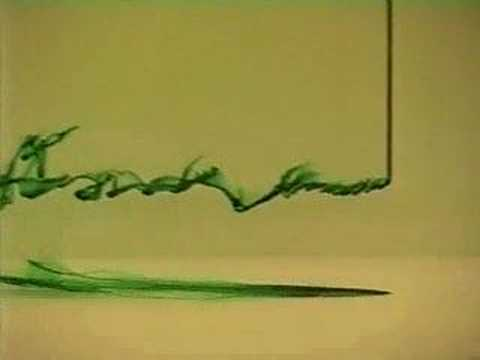
\includegraphics[scale=0.5]{simple-shear}
	\caption{No-slip condition.  \href{https://www.youtube.com/watch?v=cUTkqZeiMow&ab_channel=gurelyasin}{YouTube video.}}
\end{figure}

\noindent \textbf{Rayleigh - Pattern formation in B\'{e}nard convection}\\

I found these two images from the National Oceanic and Atmospheric Administration's (NOAA) website. The hexagons (Figure \ref{fig:RBconvec1}) appear under very delicate conditions. The flaw in the pattern (circled in red) is due to an imperfection in the plate under the fluid, which implies that the pattern is very sensitive to the boundary conditions. This also means that it is extremely unlikely to observe Rayleigh-B\'{e}nard convection patterns in our atmosphere. Figure \ref{fig:RBconvec2} shows the evolution of the pattern over a few seconds. We can see that the fluid moves up from the center of each ``cell'' and down through the walls. \\

\begin{figure}[!htb]
	\centering
	\begin{subfigure}[b]{0.45\textwidth}
		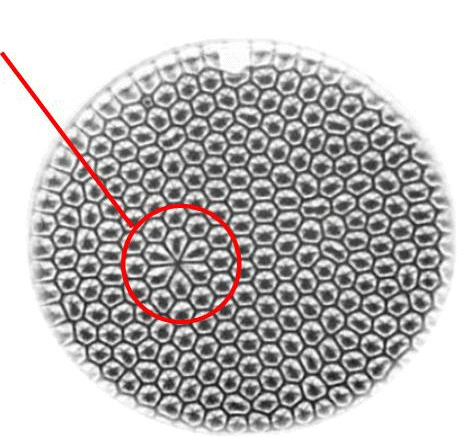
\includegraphics[width=\textwidth]{RB-convec1}
		\caption{The Burj Khalifa.}
		\label{fig:RBconvec1}
	\end{subfigure}
	\hfill
	\begin{subfigure}[b]{0.45\textwidth}
		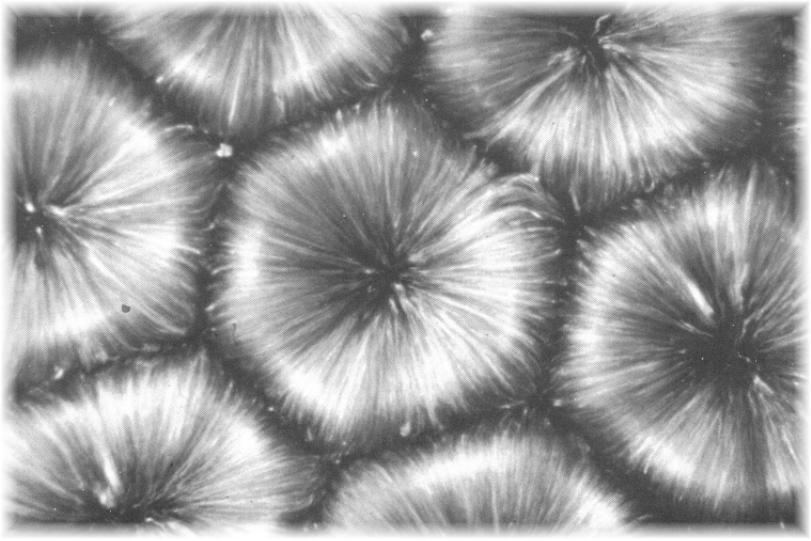
\includegraphics[width=\textwidth]{RB-convec2}
		\caption{Helical strake on a chimney.}
		\label{fig:RBconvec2}
	\end{subfigure}
\end{figure}


\begin{figure}[!htb]
	\centering
	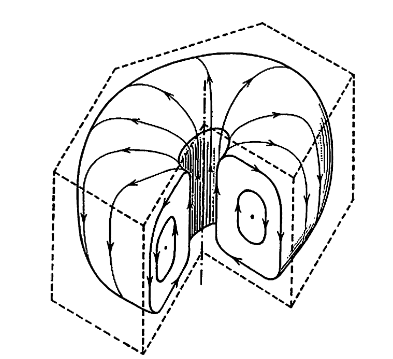
\includegraphics[scale=0.7]{RB-convec3}
	\caption{Schema of the hexagonal cellular vortex. \href{https://doi.org/10.1016/j.crme.2017.06.006}{Link to article} by J.E. Wesfreid.}
\end{figure}



\noindent \textbf{Flow around an obstacle \& K\'{a}rm\'{a}n vortex street}\\

\noindent Here, I want to look at how engineers create machines and structures that take advantage of or avoid the effects of vortex streets created by fluid flow around them. \\

A few days ago I came across this fairly recent concept of harnessing the vibrations of an obstacle due to the vortices. Figure \ref{fig:vortex1} shows a new kind of wind-power generator called Vortex Tacoma. Standing just over 3 meters tall, this new generator is bladeless and is considered by many to be a safer, quieter, and more compact alternative to traditional wind turbines. How it works is quite intuitive: given sufficiently high fluid flow (which just a fancy way of saying ``if the wind speed is big enough''), a vortex street is formed behind the mast of the generator. Since the mast is not completely fixed in place (unlike what we saw in the experiments from Tritton's book), conservation of momentum forces the mast to oscillate along with the vortices. The base of this device then transform this kinetic energy into electricity. \\

\begin{figure}[!htb]
	\centering
	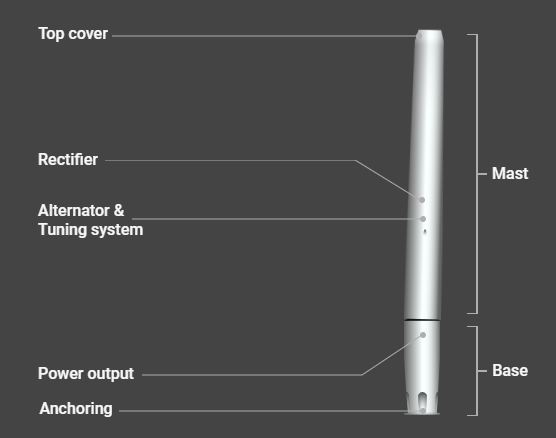
\includegraphics[scale=0.55]{vortex1}
	\caption{Schematics of Vortex Tacoma (whose name is of course inspired by the infamous collapse of the Tacoma Narrows Bridge). The design is 2.75 m tall. \href{https://vortexbladeless.com/}{Vortex Bladeless.}}
	\label{fig:vortex1}
\end{figure}

From exactly the same principles, VIVACE (Vortex Induced Vibration Aquatic Clean Energy, designed by a group of researchers at the University of Michigan) generates electricity from vortices due to water currents. Figure \ref{fig:vortex2} shows qualitatively how vortices can generate vibration. \\

\begin{figure}[!htb]
	\centering
	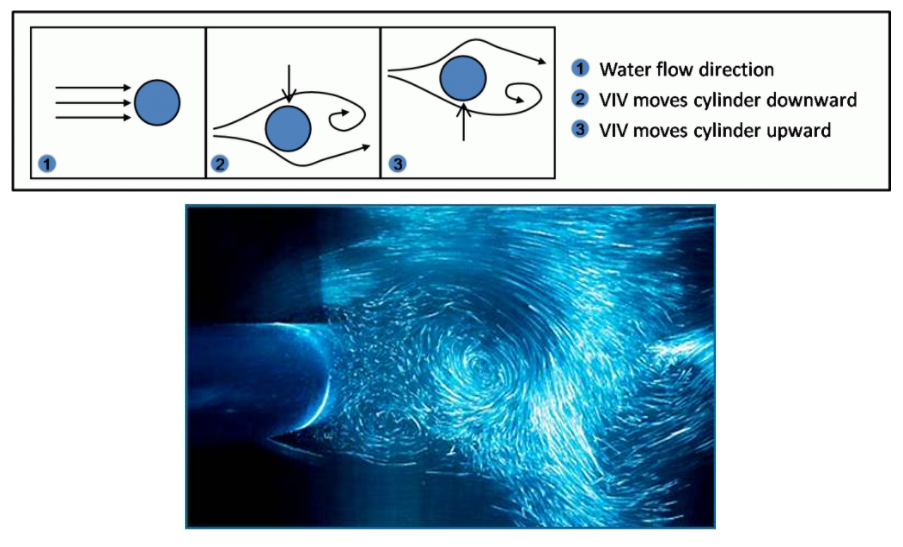
\includegraphics[scale=0.65]{vortex2}
	\caption{Vortex-induced vibration. \href{http://www.umich.edu/~mrel/}{UMich MRELab.}}
	\label{fig:vortex2}
\end{figure}

The fact that there is a significant amount of energy to harness from vortex-induced vibrations tells us that there is also a potential for destruction if we don't design our dams, bridges, and buildings carefully in terms of how they interact with water and air. The exterior of the Burj Khalifa (Figure \ref{fig:vortex3}) -- currently the world's tallest building -- is designed to disrupt any vortices from forming, since these vortices can cause the building to sway too much (or worse, swaying in resonance with the vortex ``oscillations'') \footnote{\href{https://physicstoday.scitation.org/doi/pdf/10.1063/1.3490510}{\textit{Peter Irwin, Vortices and tall buildings: A recipe for resonance},  Physics Today \textbf{63}, 9, 68 (2010); doi: 10.1063/1.3490510.}}. Another very common example of avoiding vortex-induced oscillations is the addition of a helical strake on chimneys (Figure \ref{fig:vortex4}). On the other hand, some buildings are designed to withstand the effects of vortex street formation. For example, the Willis Tower in the Windy City of Chicago, Illinois can sway up to 3 feet. 





\begin{figure}[!htb]
	\centering
	\begin{subfigure}[b]{0.45\textwidth}
		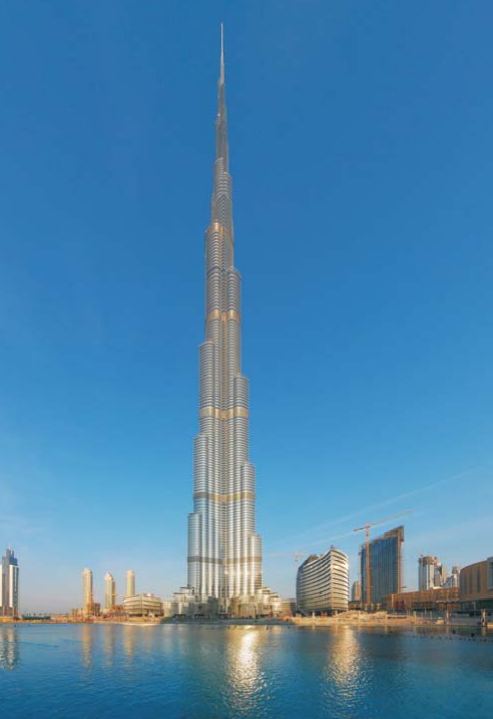
\includegraphics[width=\textwidth]{vortex3}
		\caption{The Burj Khalifa.}
		\label{fig:vortex3}
	\end{subfigure}
	\hfill
	\begin{subfigure}[b]{0.45\textwidth}
		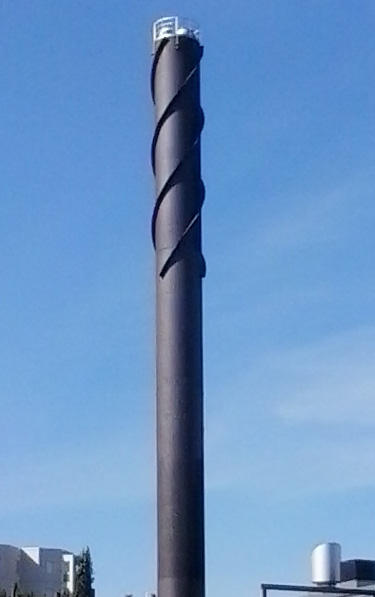
\includegraphics[width=\textwidth]{vortex4}
		\caption{Helical strake on a chimney.}
		\label{fig:vortex4}
	\end{subfigure}
\end{figure}






  
\end{document}




